\documentclass[a4paper]{IEEEtran}
\usepackage[T1]{fontenc}
\usepackage[utf8]{inputenc}
\usepackage[english]{babel}

\usepackage{authblk}
\usepackage{hyperref}
\usepackage{graphicx}
\usepackage{listings}
%\usepackage{amsmath}
\usepackage[cmex10]{amsmath}
\usepackage{amssymb}
%\usepackage{fullpage}
\usepackage{float}
\usepackage{url} \urlstyle{sf}

\usepackage{dashrule}

\usepackage{color}
\usepackage{subcaption}
\newcommand{\alert}[1]{\color{red}{#1}}
\newcommand{\greyout}[1]{\color{gray}{#1}}

\setlength{\parskip}{1em}

\title{Generating fluctuating workload for cloud elasticity simulation}
\author{
	\IEEEauthorblockN{Simon Bihel}
	\IEEEauthorblockA{(Student) Computer Science Department, ENS Rennes\\
	\href{mailto:simon.bihel@ens-rennes.fr}{simon.bihel@ens-rennes.fr}}
}


\begin{document}
\maketitle

\begin{abstract}
  Cloud computing is a model that makes available infrastructures, platforms and
  software with a pay-as-you-go subscription. It aims to reduce the cost with a
  layer of visualization that allows virtual resources to be dynamically
  adjusted and occupied on-demand. The problem of using the minimal resources
  for the current demand/usage is still a research challenge that spans all
  layers and applications. This dynamic management of clouds is called cloud
  elasticity.
\end{abstract}

\begin{IEEEkeywords}
  Simulation;
  Cloud elasticity;
  Workload
\end{IEEEkeywords}

\section{Introduction} \label{intro}


\section{Background} \label{background}
  \begin{figure*}
    \caption{http://cloud-simulation-frameworks.wikispaces.asu.edu/}
    \centering
    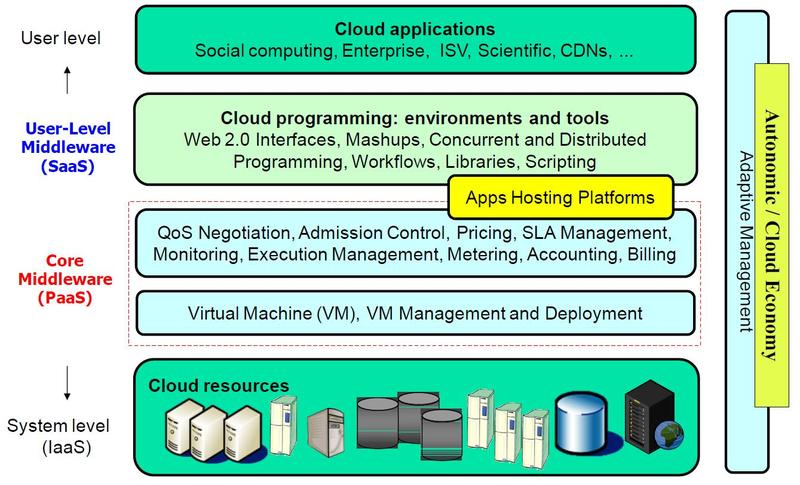
\includegraphics[width=0.7\textwidth]{../plots/cloud_architecture}
    \label{cloud_arch}
  \end{figure*}
  
  The global architecture of a cloud is described in the 
  \figurename~\ref{cloud_arch}. It is split in different layers and each layer 
  has a specific role in the business model of clouds. On the lowest part there 
  is the physical resources (e.g. data centers) with Infrastructure as a 
  Service model (Iaas). The pricing is based of the resources available. Then 
  comes the layer of virtualization and performances negotiation called 
  Platform as a Service (PaaS). Dealing with Virtual Machines (VMs) allows a 
  cleaner sharing of resources and makes it easier to answer the users' demands 
  (e.g. deploying more VMs). The pricing depends of multiple factors, like the 
  Quality of Service (QoS) for the quality of the network, the Service Level 
  Agreement (SLA) for the faults rate, handling and responsibilities... On top 
  of that is the layer for users' cloud tools with Software as a Service 
  (SaaS). These tools will allow the user that writes cloud applications to 
  manage resources, run their code...
  
  Most cloud applications will have fluctuating workload over time. For exemple 
  with a website server the usage might be bigger during the day or during a 
  short period because of a viral cultural event. Resources should thus be 
  managed dynamically. Also, physical resources can encounter problems which 
  makes them unavailable. Because of all these constraints the SLAs and QoS 
  negotiations aren't satisfied easily and 100\% availability is never a thing. 
  On top of that every actor wants to meet the obligations with a minimal cost. 
  All these questions of availability and cost are current research problems. 
  In particular we are interested in the works that tackle problems related to 
  fluctuating and dynamic usage of cloud applications and resources. The 
  ability for a cloud infrastructure to adapt to a dynamic workload is called 
  cloud elasticity.
  
  There are some generic elastic actions. The act of deploying more VMs (and
  thus having more resources overall) is called scaling up (and the convert is
  scaling down). The act of moving VMs to a different location is called scaling
  out. This is used for example when time passes by and users come from
  different countries/continents.
  
  \cite{Naskos2016} has categorized works on cloud elasticity and allows to see
  which elements of a cloud infrastructure, platform or application/software are
  impacted. As it is for now most research works are evaluated on real clouds It
  is interesting for a distributed systems simulator to search what is needed
  for simulating cloud elasticity. If it is shown that research works on cloud
  elasticity can be evaluated on a simulator they would benefit from cost
  reduction, re-runable experiments, trust in results...
  
  In this survey proposals are categorized as follows. The scope is about what
  elements of a cloud the proposals work on. It can be the management of VMs,
  allocation of resources... Then there is the purpose of the proposal.
  Enhancing the \textit{performances} (to meet the SLA), reducing the
  \textit{energy consumption} footprint, being \textit{available} when needed
  and reducing the overall \textit{cost}. Another dimension is the decision
  making. This is what a proposal add to an existing cloud to pursue its
  purpose. In addition to the scope there is the elastic actions performed by
  the proposals. As the scope is about what elements of a cloud are concerned,
  the elastic action is about what is done to them. Then there is the provider
  dimension that tells if there is only one provider or multiple ones. At last
  there is the method used by the proposal to evaluate itself, through real
  cloud, simulation or emulation.
  
  The survey gives a good overview on what elements of a cloud are
  manipulated to achieve cloud elasticity. No clue have been found to prove the 
  opposite at the time of writing.
  
  As the proposals are on reacting to variating usage, simulators need a way to
  express this fluctuating workload. We worked on elastic tasks that model tasks
  that are triggered regularly and with a usage that fluctuates over time.


\section{State of the art} \label{sota}
  \begin{itemize}
    \item Which elements have to be simulated and how do they work ?
    \item How workloads are generally modelized
    \item What others simulators have done
    \item What simulations for evaluation have been done
    \item What others evaluations do
  \end{itemize}
  
  Based on the classification of the survey, a simulator should allow the
  manipulation of scopes, the evaluation of the different purposes, make
  possible the elastic actions and allow multiple providers.
  
  At the moment no simulator article talks about dynamic workload. On the other
  hand in the code of DCsim \cite{tighe2013towards} there was an interactive
  task and in the code of CloudSim \cite{calheiros2011cloudsim} there was an
  host with dynamic workload.


\section{Contribution} \label{contrib}
  What can my contribution do that is in the survey?
  \begin{itemize}
    \item Only computational tasks for now, might be able to do storage/DBs
    tasks in the future. Generic ones won't be possible unless you can pass a
    task directly to an ET.
    \item Need to use the host of a task when executing to allow vertical
    scaling and need to manage multiple hosts to allow horizontal scaling.
    \item Multiple provider is possible but has to be coded.
    \item Purpose?
  \end{itemize}
  
  The work was done on SimGrid \cite{casanova:hal-01017319}.


\section{Evaluation} \label{eval}
  The contribution has been evaluated on the predefined criteria. We first did 
  an experiment for raw performances. Then we used real traces from WorldCup 98 
  data access logs \cite{wc98} which are often used. After that we evaluated 
  the expressiveness and functionalities. All experiments have been executed on 
  a MacBook Pro with an Intel Core i5 and 8GB of RAM.
    
  \subsection{Raw performances}
    \begin{figure}
      \caption{Raw performances CPU time}
      \centering
      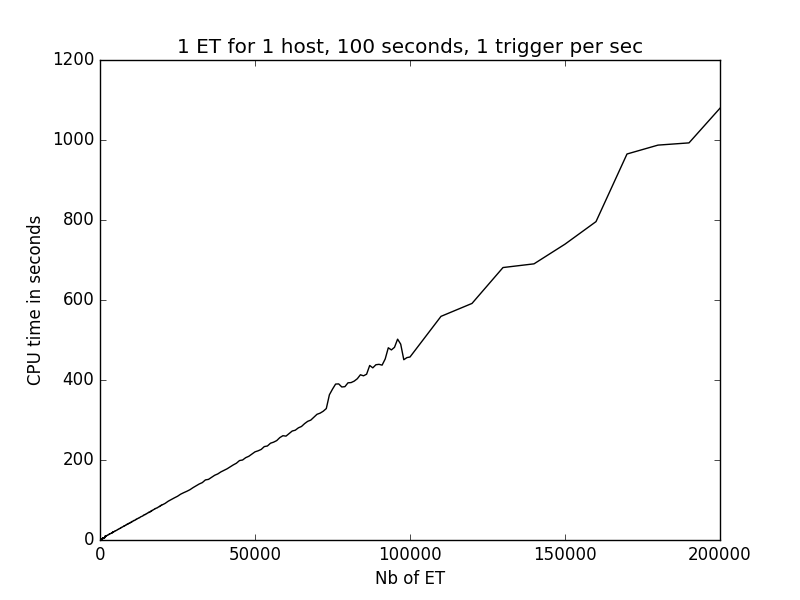
\includegraphics[width=0.55\textwidth]{../plots/raw_perf_time}
      \label{time_raw}
    \end{figure}
    \begin{figure}
      \caption{Raw performances Max Memory}
      \centering
      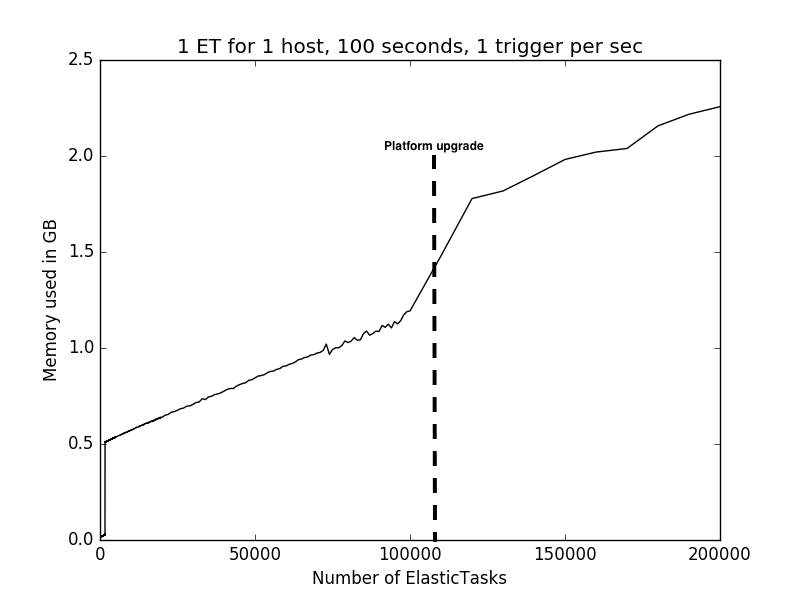
\includegraphics[width=0.55\textwidth]{../plots/raw_perf_mem}
      \label{mem_raw}
    \end{figure}
    
    \figurename~\ref{time_raw} shows the CPU time (user + system time) while 
    \figurename~\ref{mem_raw} shows the maximum memory used. The platform was
    upgraded two times, at 1,600 from 2,000 hosts to 100,000, and then at
    100,000 from 100,000 to 200,000.
    
    % for the spikes in CPU it might be because I was doing other stuff with my 
    % laptop
    
  \subsection{Real traces}
  
  \subsection{Functionalities}
  

\section{Future work} \label{futurework}
% generator law
  

\section{Conclusion} \label{conclu}



\bibliographystyle{IEEEtran}
\bibliography{bibi}
\end{document}
